\newpage
\section{Operating-System Structure}

\subsection{Operating System Services}
For user
\begin{itemize}
    \item User interface (UI): Command-Line(CLI), Graphics User Interface (GUI)
    \item Programe execution
    \item I/O operations
    \item File-system manipulation
    \item Communications 
    \item Error detection
\end{itemize}

For system
\begin{itemize}
    \item Resource allocation
    \item Accounting
    \item Protection and security
\end{itemize}

\subsection{System Call}
使用高级语言写 system call. 

Application Program Interface (API) 与 system call 看作是不同的, API 层级更高. 

POSIX API 标准化了 API.

\subsubsection{Implementation}
每个 system call 会有一个 number. System-call interface 维护一个 number 索引的 table. 

封装 好处: 抽象, 可移植 etc.

\begin{figure}[!htb]
    \centering
    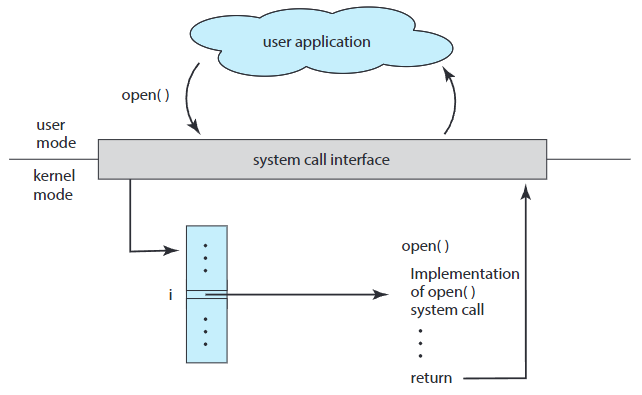
\includegraphics[width=0.42\textwidth]{pic/OS2/API – System Call – OS Relationship}
    \caption{API – System Call – OS Relationship}
\end{figure}

\subsubsection{Parameter Passing}
Three general methods used to pass parameters to the OS: 
\begin{itemize}
    \item Simplest: pass the parameters in \textbf{registers}. 但有时不够用. 
    \item Parameters stored in a \textbf{block}, or table, in memory, and address of block passed as a parameter in a register. 
    \item Parameters placed, or pushed, onto the \textbf{stack} by the program and popped off the stack by the operating system. 
\end{itemize}
Block and stack methods do not limit the number or length of parameters being passed. 


\subsection{Types of System Calls}

\begin{itemize}
    \item Process control
    \item File management
    \item Device management
    \item Information maintenance (e.g. time, date)
    \item Communications
    \item Protection    
\end{itemize}


\subsection{System Programs}
System programs provide a convenient environment for program development and execution. They can be divided into:
\begin{itemize}
    \item File manipulation
    \item Status information
    \item File modification
    \item Programming language support
    \item Program loading and execution
    \item Communications
    \item Application programs
\end{itemize}


\subsection{Operating System Design and Implementation}
OS设计与实现没有明确输入输出. Start by defining goals and specifications. Affected by choice of hardware, type of system. 

\begin{itemize}
    \item User goals --- operating system should be convenient to use, easy to learn, reliable, safe, and fast
    \item System goals --- operating system should be easy to design, implement, and maintain, as well as flexible, reliable, error-free, and efficient
\end{itemize}


\subsubsection{Mechanism and Policy} %TODO 读 2.7.2 P80
Important principle to separate: (分离策略与机制)
\begin{itemize}
    \item Policy: What will be done? 策略(确定具体做什么事, 部分输入信息)
    \item Mechanism: How to do it? 机制(定义做事方式, 模型)
\end{itemize}

\subsection{Operating System Structure}

\subsubsection{Layered Approach}
仅帮助人类理解. 
\begin{figure}[!htb]
    \centering
    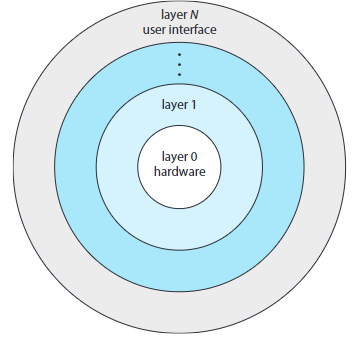
\includegraphics[width=0.22\textwidth]{pic/OS2/Layered Operating System}
    \caption{Layered Operating System}
\end{figure}

\subsubsection{Monolithic structure}
(宏内核) e.g. UNIX
\begin{figure}[!htb]
    \centering
    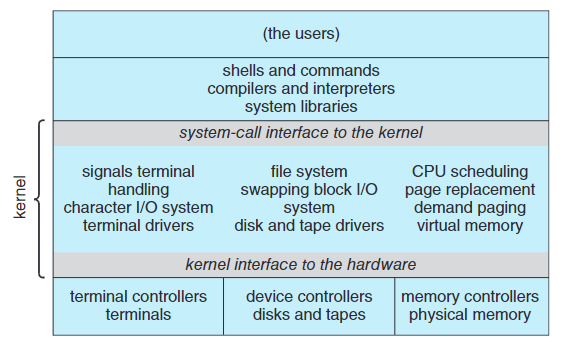
\includegraphics[width=0.42\textwidth]{pic/OS2/Traditional UNIX system structure}
    \caption{Traditional UNIX system structure}
\end{figure}

\subsubsection{Microkernel System Structure}
(微内核) 把很多操作分到 user code 之中. 
Benefits: 代码少, 稳定, 易移植. 
Detriments: 效率变低 (Performance overhead). 


\begin{figure}[!htb]
    \centering
    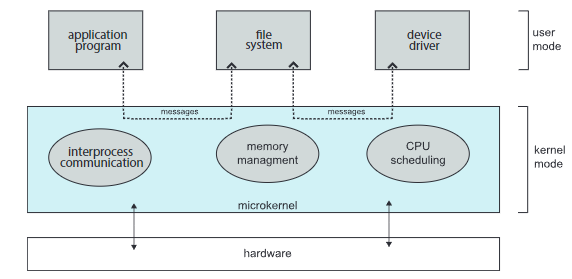
\includegraphics[width=0.42\textwidth]{pic/OS2/Architecture of A Typical Microkernel}
    \caption{Architecture of A Typical Microkernel}
\end{figure}

\subsubsection{Kernel Modules}
(内核模块) 现代常用. 提供扩展内核的能力(loadable kernel modules, LKM). 

\subsubsection{Other Structures}
\paragraph{Exokernel} (外核) 高度简化kernel, 只负责资源分配, 提供了低级的硬件操作, 必须通过定制library供应用使用. 高性能, 但定制化library难度大, 兼容性差. 

\begin{figure}[!htb]
    \centering
    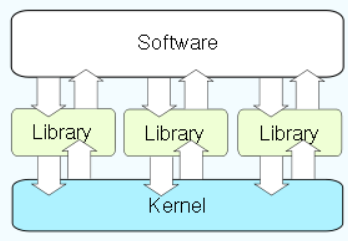
\includegraphics[width=0.22\textwidth]{pic/OS2/Exokernel.png}
    \caption{Exokernel}
\end{figure}

\paragraph{Unikernel} (单核), 来自 include OS. 静态连接所有的 OS 代码. 适用于云服务, app 的 boots, 启动耗时只需几十ms. 达到\textbf{高可用}.  

\begin{figure}[!htb]
    \centering
    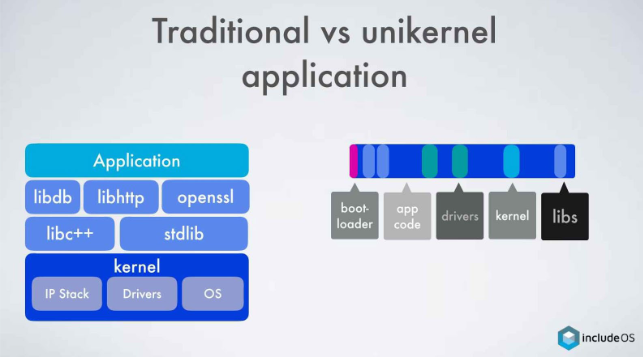
\includegraphics[width=0.42\textwidth]{pic/OS2/Unikernel.png}
    \caption{Unikernel}
\end{figure}


\subsection{Virtual Machines}
(虚拟机) 虚拟机算是分层方法的自然结果. 其把底层的硬件与OS都视为自己的硬件. 有全虚拟化(解释执行) 与 物理虚拟化(底层执行). 

\begin{figure}[!htb]
    \centering
    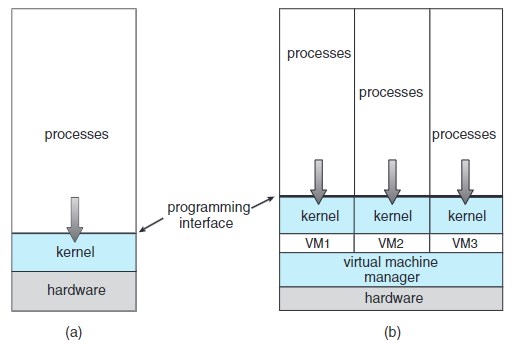
\includegraphics[width=0.42\textwidth]{pic/OS2/virtual machines..png}
    \caption{A computer running (a) a single operating system and (b) three virtual machines.}
\end{figure}

\begin{figure}[!htb]
    \centering
    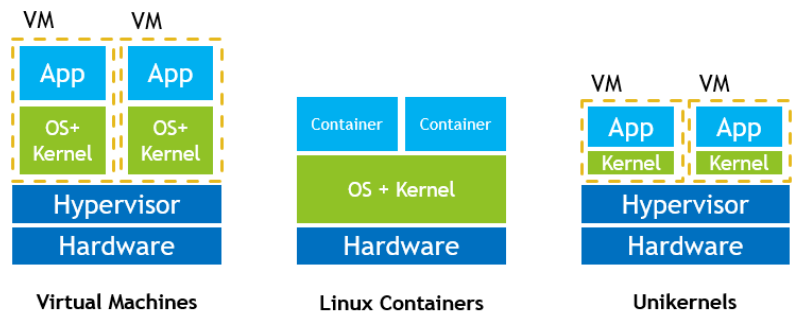
\includegraphics[width=0.42\textwidth]{pic/OS2/Different Techniques}
    \caption{Different Techniques}
\end{figure}
\newpage
\quad



